\documentclass[../psets.tex]{subfiles}

\pagestyle{main}
\renewcommand{\leftmark}{Problem Set \thesection}
\stepcounter{section}

\begin{document}




\section{Reactive Intermediates}
\marginnote{10/16:}The questions pertain to the material covered from Cations (Sep 24) to Selectivity (Oct 8).
\begin{enumerate}
    \item The radicals below are known to be \textbf{bench-stable}, meaning they don't readily dimerize or get quenched by oxygen. Rationalize this observation for each.
    \begin{center}
        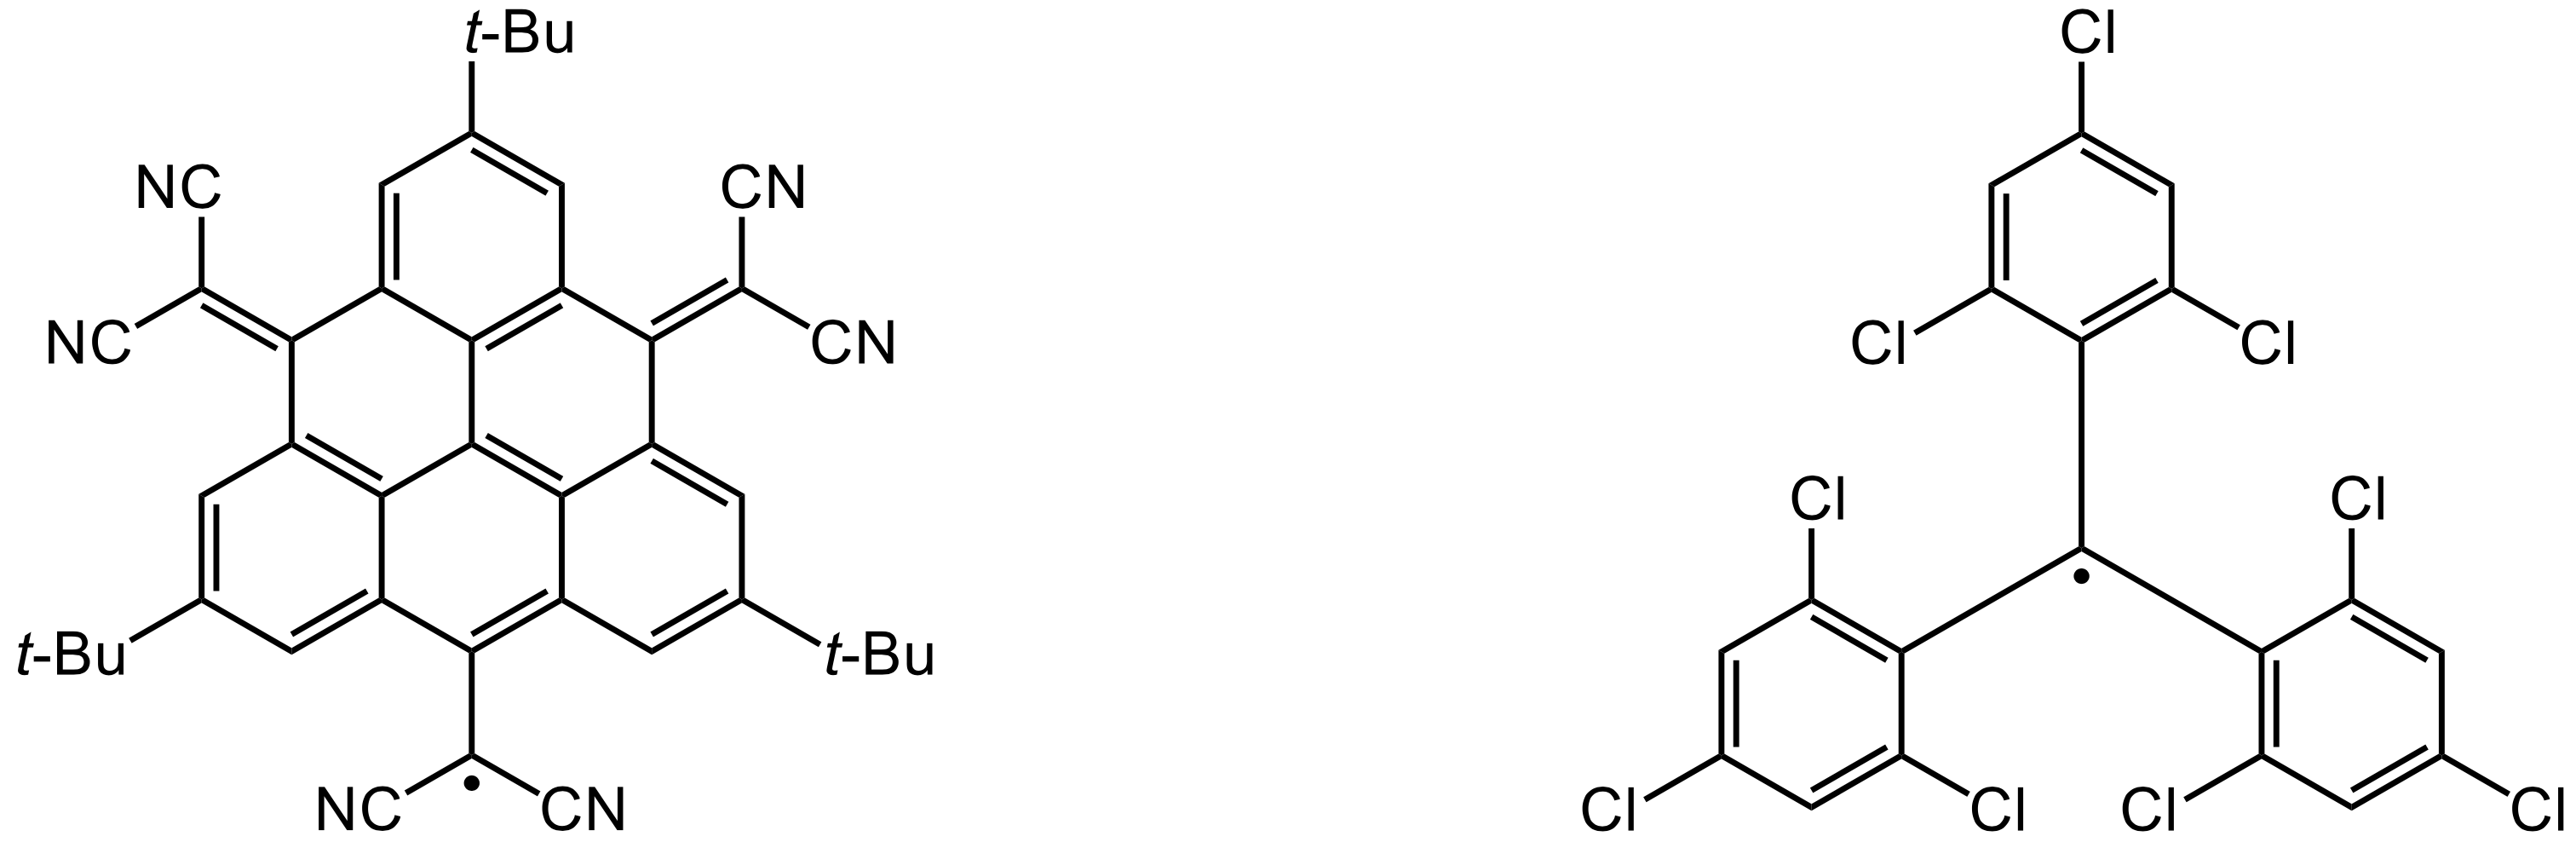
\includegraphics[width=0.8\linewidth]{PSet2F1.png}
    \end{center}
    \item 
    \begin{enumerate}
        \item Propose a reasonable arrow-pushing mechanism that explains the formation of the major product in the reaction below.
        \begin{center}
            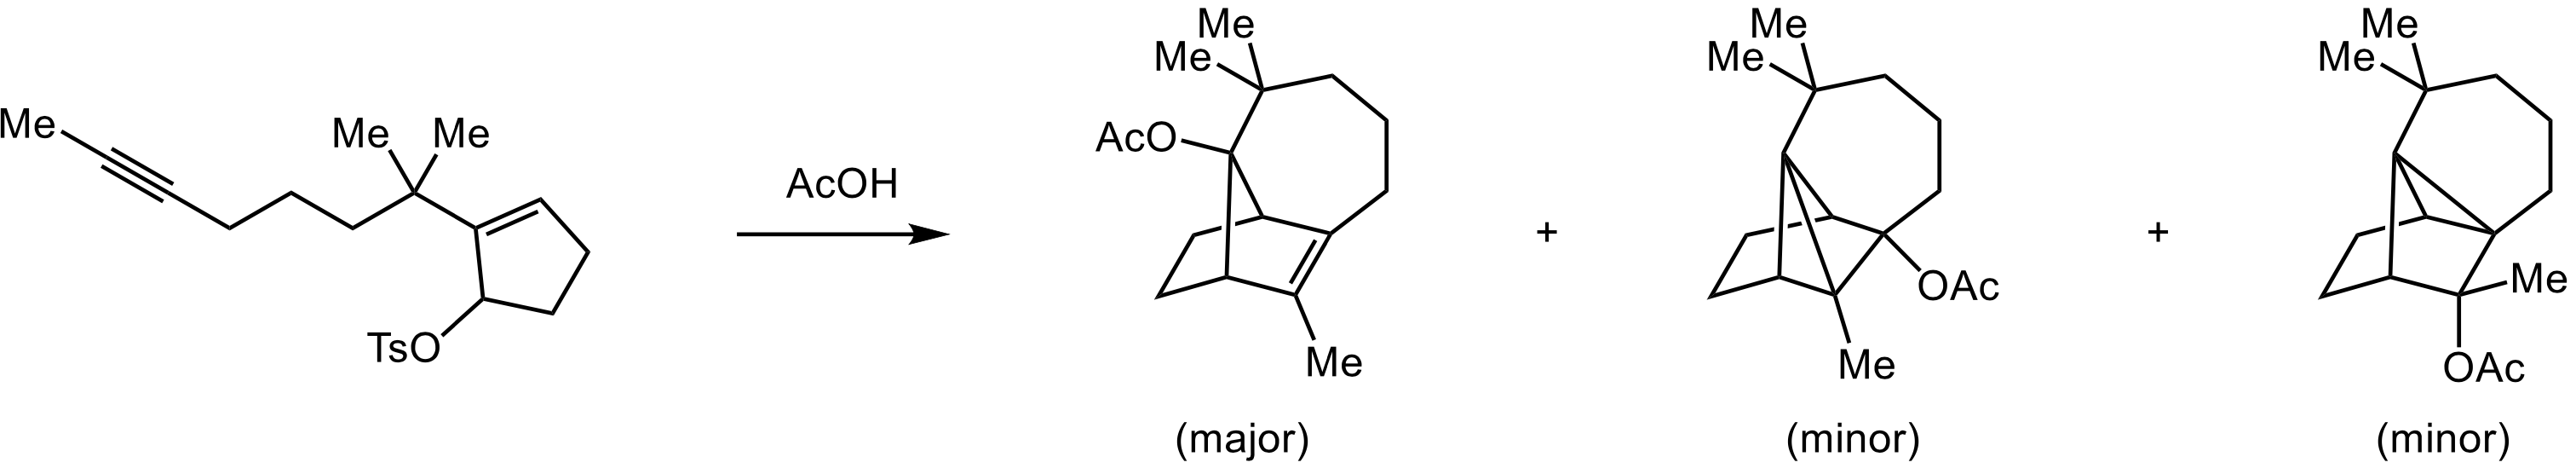
\includegraphics[width=0.95\linewidth]{PSet2F2.png}
        \end{center}
        \item Suggest how the minor products could be formed and draw the key intermediate(s) involved.
    \end{enumerate}
    \item Which of the following two compounds is more acidic (lower $\pKa$)? Compare the acidity of the protons indicated red. Rationalize your answer.
    \begin{enumerate}
        \item {\color{white}hi}
        \begin{center}
            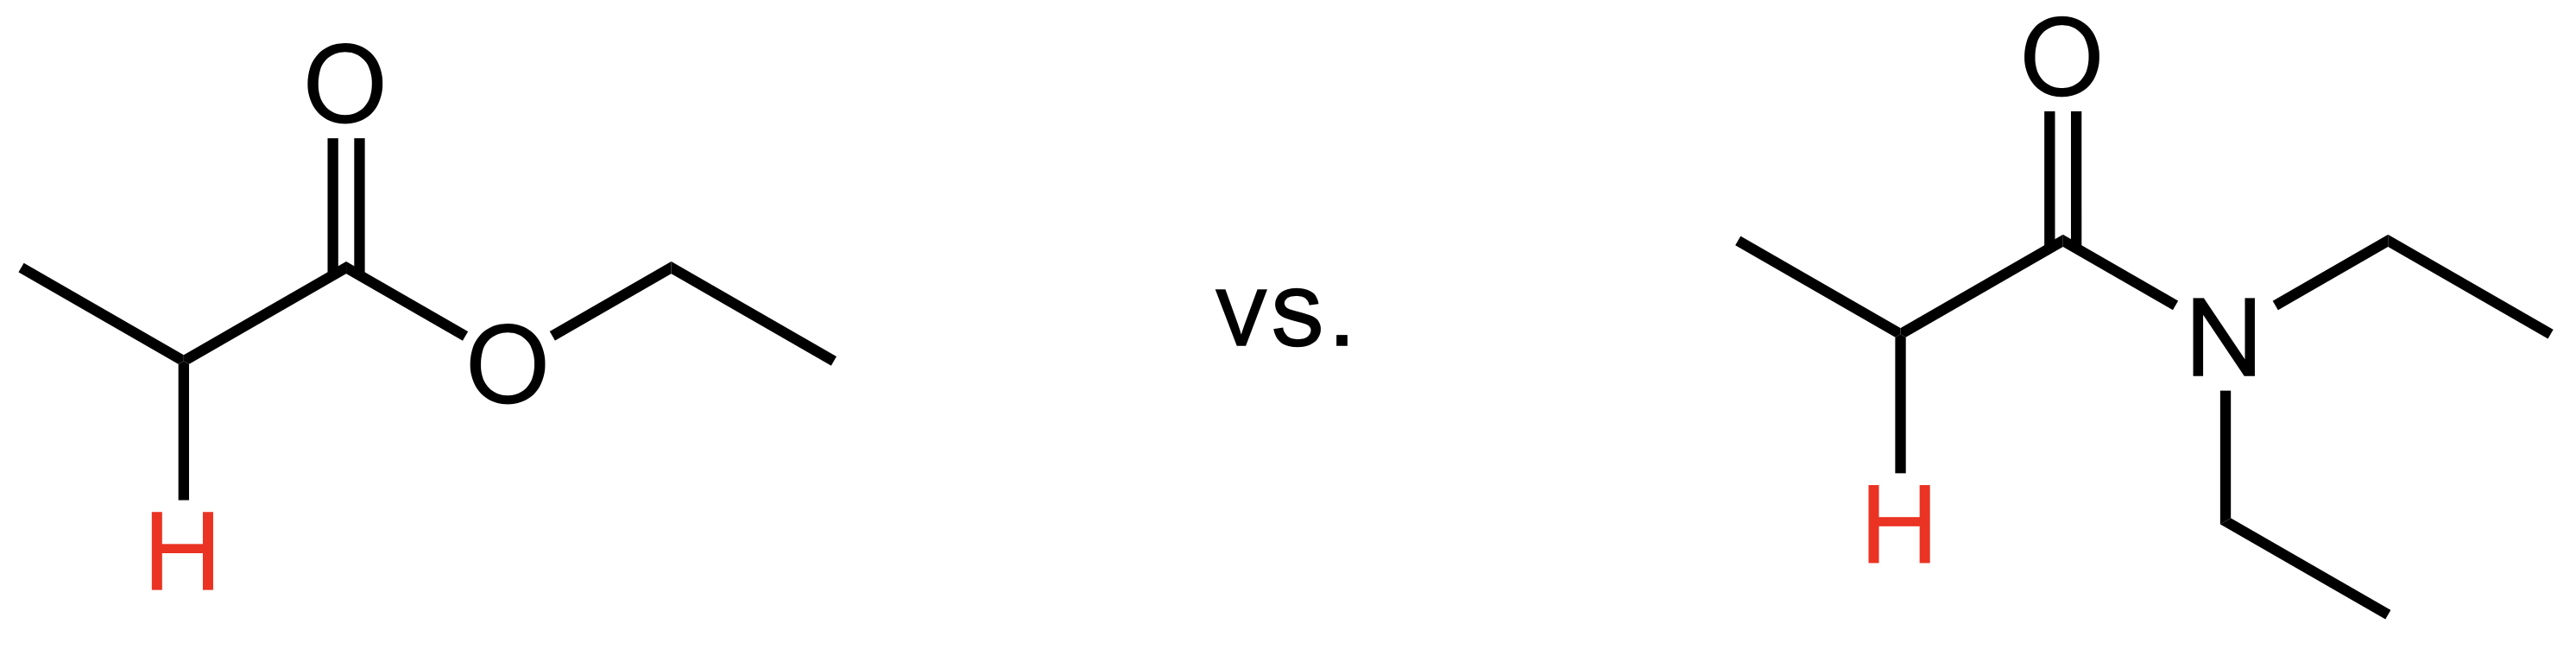
\includegraphics[width=0.45\linewidth]{PSet2F3.png}
        \end{center}
        \item {\color{white}hi}
        \begin{center}
            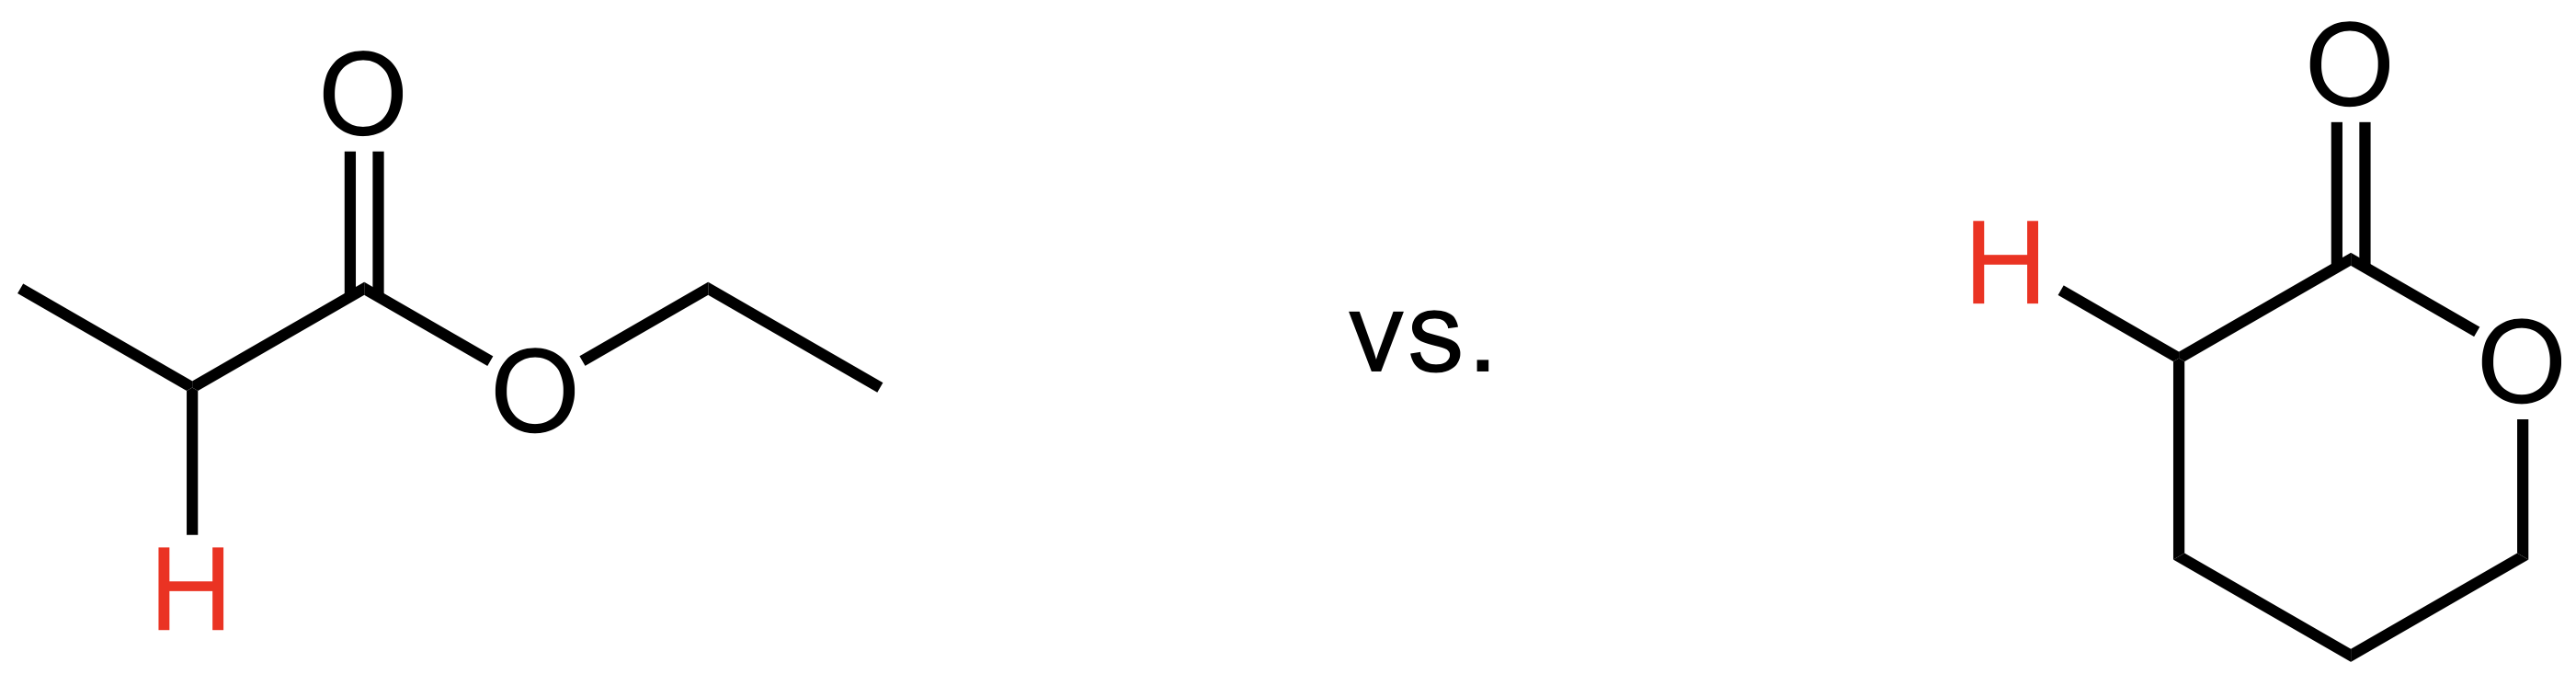
\includegraphics[width=0.45\linewidth]{PSet2F4.png}
        \end{center}
    \end{enumerate}
    \item 
    \begin{enumerate}
        \item Suggest a reasonable mechanism for the following transformation.
        \begin{center}
            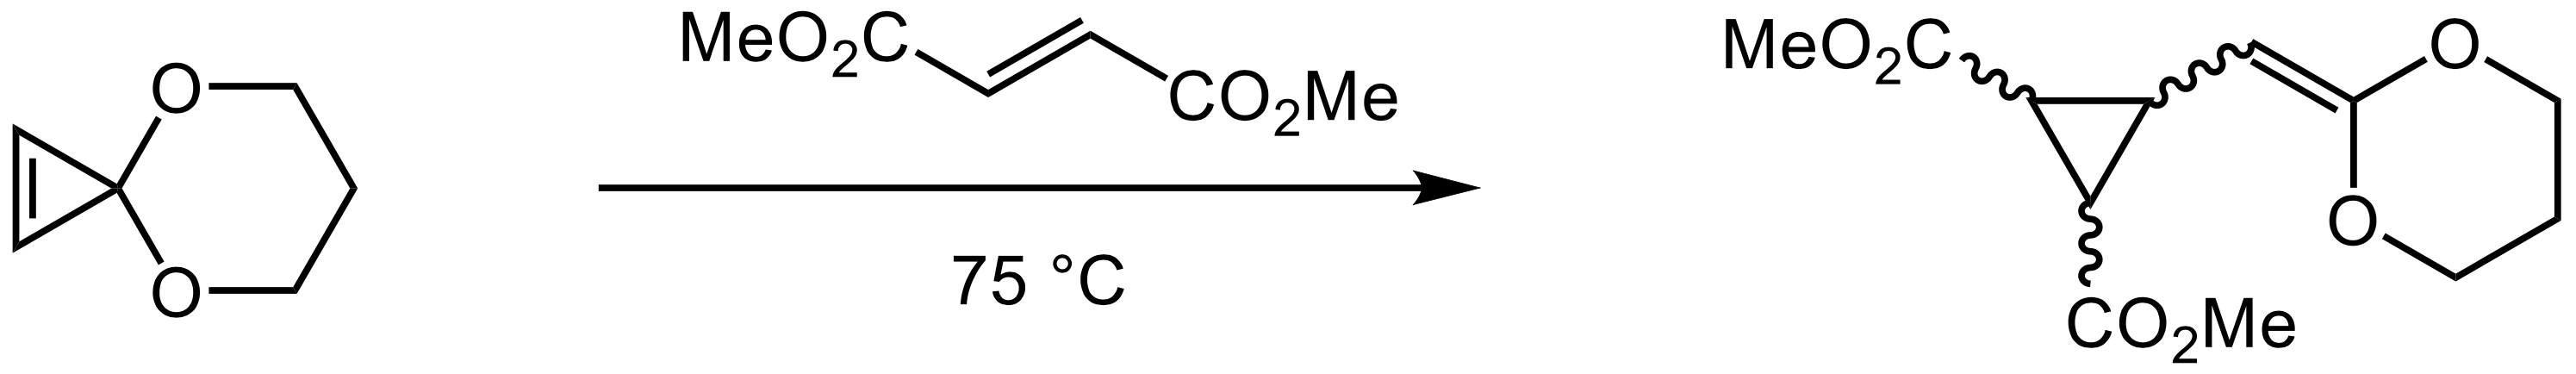
\includegraphics[width=0.7\linewidth]{PSet2F5.png}
        \end{center}
        \item Discuss the stability of the intermediate(s) and predict the stereochemistry of the product.
    \end{enumerate}
    \pagebreak
    \item Draw potential energy diagrams for each of the following situations. Use dashed horizontal lines to indicate equivalent energy levels.
    \begin{enumerate}
        \item A single substrate can undergo two reactions with equal rates but different product stabilities. What reaction conditions would you use if you wanted a mixture of products? What reaction conditions would you use if you wanted a single product, and which product would you expect?
        \item The formation of a kinetically stable radical from a precursor and dimerization of that radical.
        \item The stereoselective protonation of a tertiary carbanion.
        \item Starting from one pure diastereomer, the epimerization of the alpha position of a ketone under acidic conditions to form a mixture of products.
    \end{enumerate}
\end{enumerate}




\end{document}